% Object-Centric VQ Encoder — Architecture Diagram
% Compile: pdflatex architecture_oc_encoder.tex
%
% To embed in a paper, copy everything inside \begin{tikzpicture}...\end{tikzpicture}
% and add to your preamble:
%   \usepackage{tikz}
%   \usetikzlibrary{arrows.meta,positioning,calc,backgrounds}
%   \usepackage{amsmath}

\documentclass[tikz,border=10pt]{standalone}
\usepackage{tikz}
\usetikzlibrary{arrows.meta, positioning, calc, backgrounds}
\usepackage{amsmath}

%% ── Colours ────────────────────────────────────────────────────────────────
\definecolor{Cobs}{HTML}{DCE8F5}    % input
\definecolor{Cemb}{HTML}{E8F4E8}    % embedding / tokenise
\definecolor{Ctrf}{HTML}{FFF3CD}    % transformer
\definecolor{Cagt}{HTML}{D4E6F1}    % agent head
\definecolor{Ckey}{HTML}{FDE8D8}    % key head
\definecolor{Cdor}{HTML}{E8F5E9}    % door head
\definecolor{Cvq} {HTML}{F5E6FA}    % VQ layer
\definecolor{Ccat}{HTML}{EEEEEE}    % concat / policy output
\definecolor{Cdec}{HTML}{F8F8F8}    % decoder (training only)
\definecolor{Clss}{HTML}{FFF0F0}    % loss box
\definecolor{Cblu}{HTML}{2C6FAD}    % agent accent
\definecolor{Corg}{HTML}{C45F1A}    % key accent
\definecolor{Cgrn}{HTML}{2E7D32}    % door accent
\definecolor{Cpur}{HTML}{6A1B9A}    % VQ annotation
\definecolor{Cgry}{HTML}{888888}    % secondary / dashes
\definecolor{Cedg}{HTML}{333333}    % default edge

%% ── TikZ styles ─────────────────────────────────────────────────────────────
\tikzset{
  %% Full-width backbone block (obs, emb, tok, trf, cat)
  bbone/.style={
    draw=Cedg, fill=#1, rounded corners=3pt,
    minimum width=10.6cm, inner sep=6pt,
    align=center, font=\small, line width=0.75pt,
  },
  bbone/.default=white,
  %% Per-head column boxes — one style per head (avoids n-arg style)
  abox/.style={draw=Cblu, fill=Cagt, rounded corners=3pt,
    minimum width=3.0cm, inner sep=5pt, align=center,
    font=\small, line width=1.1pt},
  kbox/.style={draw=Corg, fill=Ckey, rounded corners=3pt,
    minimum width=3.0cm, inner sep=5pt, align=center,
    font=\small, line width=1.1pt},
  dbox/.style={draw=Cgrn, fill=Cdor, rounded corners=3pt,
    minimum width=3.0cm, inner sep=5pt, align=center,
    font=\small, line width=1.1pt},
  %% VQ boxes — one per head
  avq/.style={draw=Cblu, fill=Cvq, rounded corners=3pt,
    minimum width=3.0cm, minimum height=1.5cm, inner sep=5pt,
    align=center, font=\small\bfseries, line width=1.4pt},
  kvq/.style={draw=Corg, fill=Cvq, rounded corners=3pt,
    minimum width=3.0cm, minimum height=1.5cm, inner sep=5pt,
    align=center, font=\small\bfseries, line width=1.4pt},
  dvq/.style={draw=Cgrn, fill=Cvq, rounded corners=3pt,
    minimum width=3.0cm, minimum height=1.5cm, inner sep=5pt,
    align=center, font=\small\bfseries, line width=1.4pt},
  %% Dashed training-only box
  tbox/.style={
    draw=Cgry, fill=Cdec, rounded corners=3pt, dashed,
    minimum width=#1, inner sep=5pt,
    align=center, font=\small, line width=0.7pt,
  },
  tbox/.default=3.5cm,
  %% Arrows
  marr/.style={-{Stealth[length=5pt,width=4pt]},
               draw=Cedg, line width=0.8pt},
  darr/.style={-{Stealth[length=4pt,width=3pt]},
               draw=Cgry, line width=0.7pt, dashed},
  %% Coloured solid arrow (used as [carr=Cblu])
  carr/.style={-{Stealth[length=5pt,width=4pt]},
               draw=#1, line width=0.9pt},
  %% Coloured dashed arrow (used as [dcarr=Corg])
  dcarr/.style={-{Stealth[length=4pt,width=3pt]},
                draw=#1, line width=0.7pt, dashed},
}

%% ── Column x-offsets from backbone centre ──────────────────────────────────
\newcommand{\Xa}{-3.6cm}   % agent column
\newcommand{\Xd}{ 3.6cm}   % door column

\begin{document}
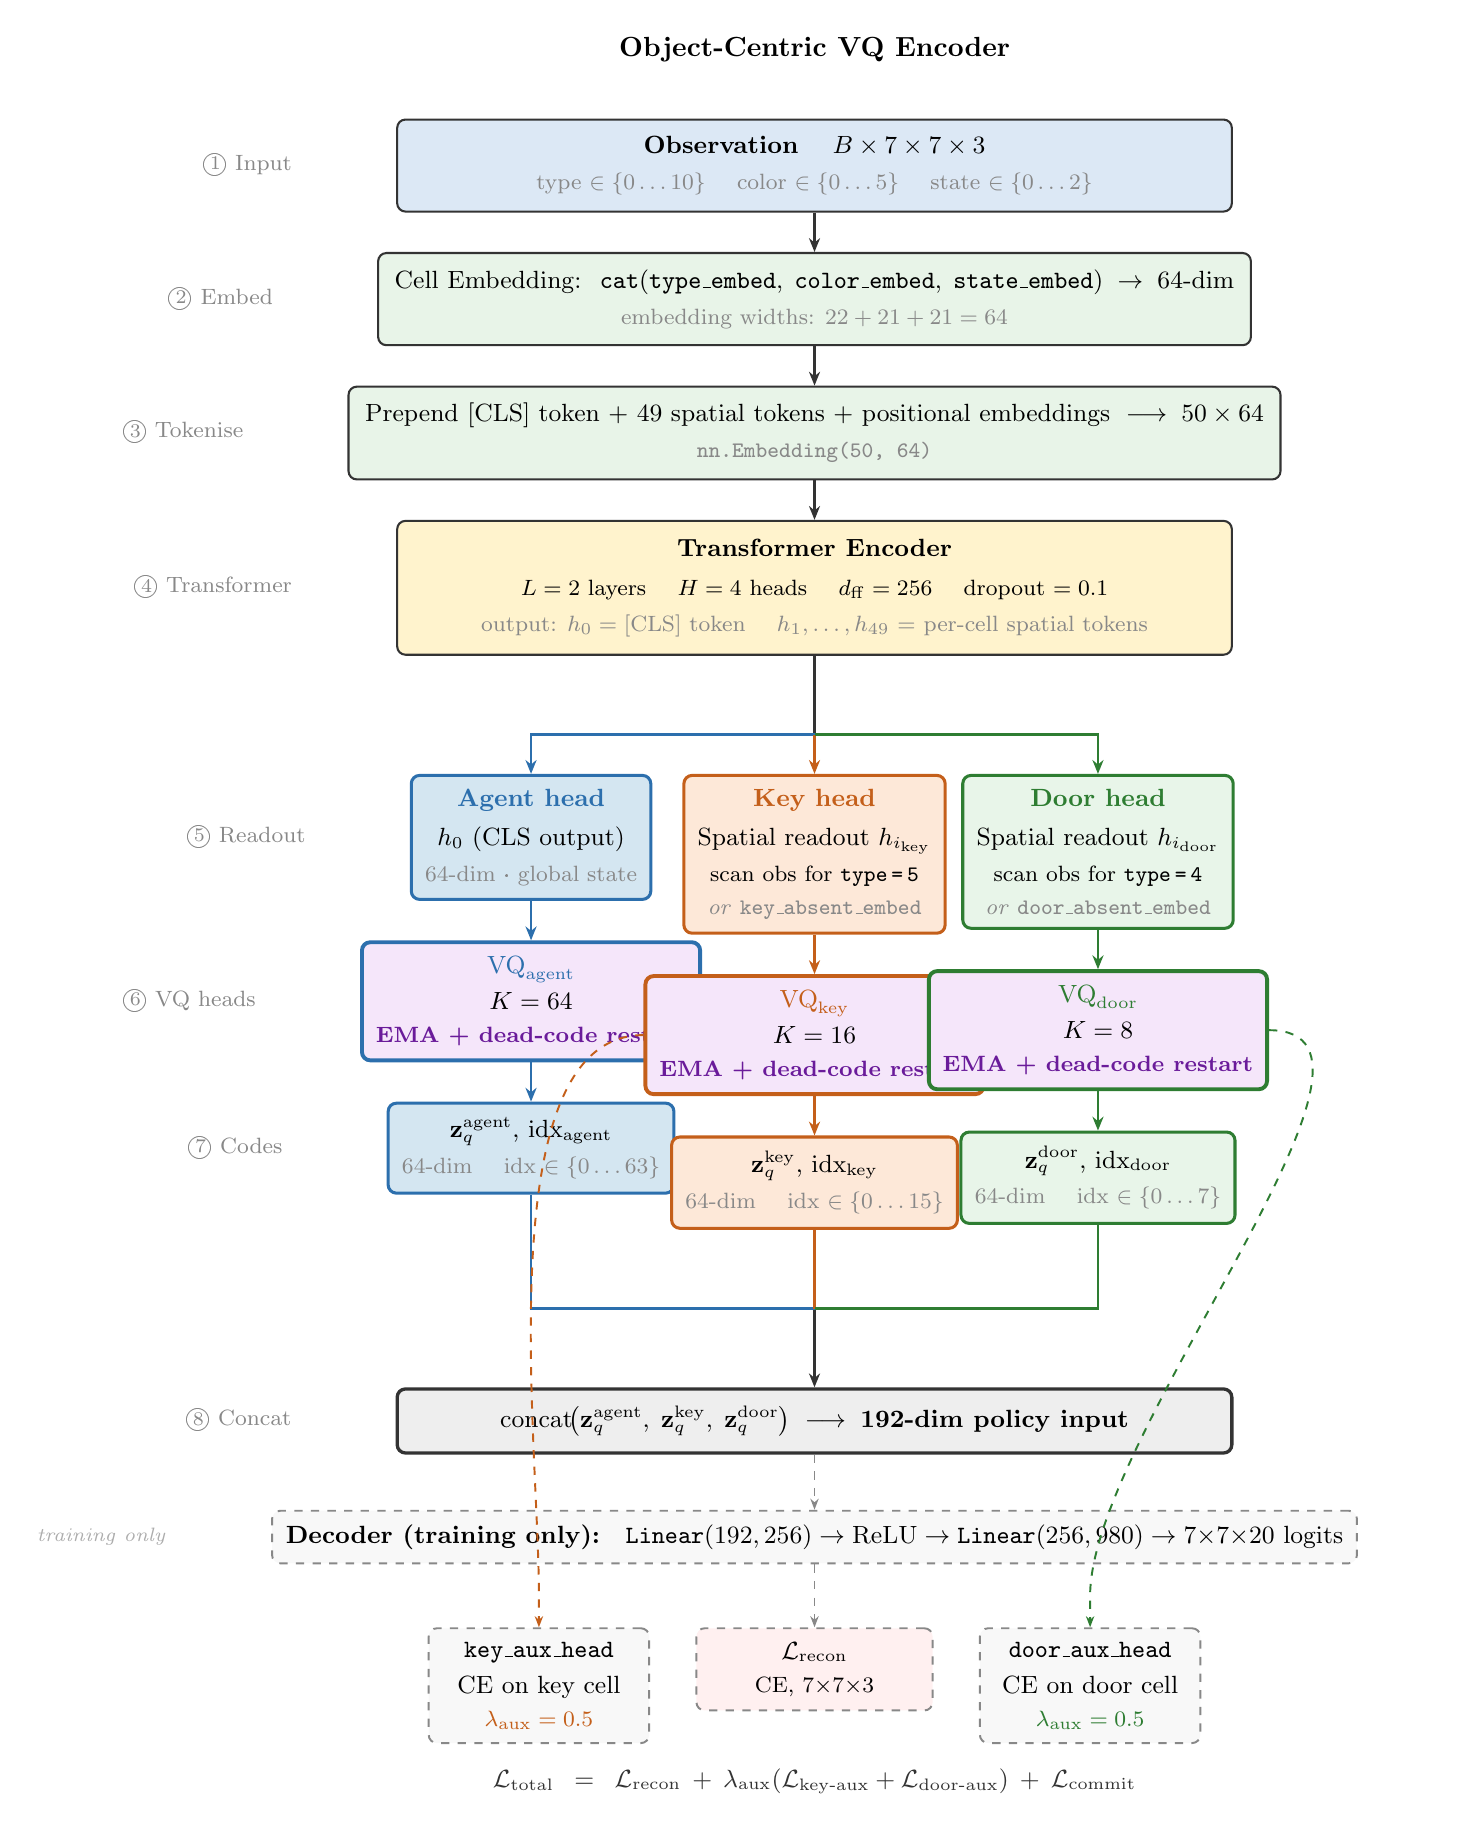
\begin{tikzpicture}[node distance=5mm]

%% ═══════════════════════════════════════════════════════════════════════════
%% TITLE
%% ═══════════════════════════════════════════════════════════════════════════
\node[font=\normalsize\bfseries] (title) {Object-Centric VQ Encoder};

%% ═══════════════════════════════════════════════════════════════════════════
%% BACKBONE — top section
%% ═══════════════════════════════════════════════════════════════════════════

\node[bbone=Cobs, below=6mm of title] (obs) {%
  \textbf{Observation} \quad $B \times 7 \times 7 \times 3$ \\[2pt]
  {\color{Cgry}\footnotesize
    type $\in \{0\ldots10\}$ \quad color $\in \{0\ldots5\}$ \quad
    state $\in \{0\ldots2\}$}%
};

\node[bbone=Cemb, below=5mm of obs] (emb) {%
  Cell Embedding:\;
  $\texttt{cat}(\texttt{type\_embed},\;\texttt{color\_embed},\;\texttt{state\_embed})
  \;\to\; 64\text{-dim}$ \\[2pt]
  {\color{Cgry}\footnotesize embedding widths: $22 + 21 + 21 = 64$}%
};

\node[bbone=Cemb, below=5mm of emb] (tok) {%
  Prepend $[\mathrm{CLS}]$ token $+$ 49 spatial tokens
  $+$ positional embeddings $\;\longrightarrow\; 50 \times 64$ \\[2pt]
  {\color{Cgry}\footnotesize \texttt{nn.Embedding(50, 64)}}%
};

\node[bbone=Ctrf, below=5mm of tok, minimum height=1.7cm] (trf) {%
  \textbf{Transformer Encoder} \\[3pt]
  {\footnotesize $L = 2$ layers \quad $H = 4$ heads \quad
    $d_{\mathrm{ff}} = 256$ \quad dropout $= 0.1$} \\[2pt]
  {\color{Cgry}\footnotesize
    output: $h_0 = \text{[CLS] token}$ \quad
    $h_1, \ldots, h_{49}$ = per-cell spatial tokens}%
};

%% ═══════════════════════════════════════════════════════════════════════════
%% THREE-HEAD SECTION — readout, VQ, codes
%% ═══════════════════════════════════════════════════════════════════════════

%% Readout boxes (1.5 cm below transformer bottom)
\node[abox, below=1.5cm of trf, xshift=\Xa] (ro_a) {%
  \textcolor{Cblu}{\textbf{Agent head}} \\[3pt]
  $h_0$ (CLS output) \\[2pt]
  {\color{Cgry}\footnotesize 64-dim · global state}%
};

\node[kbox, below=1.5cm of trf] (ro_k) {%
  \textcolor{Corg}{\textbf{Key head}} \\[3pt]
  Spatial readout $h_{i_{\mathrm{key}}}$ \\[2pt]
  {\footnotesize scan obs for \texttt{type\,=\,5}} \\[1pt]
  {\color{Cgry}\footnotesize \textit{or} \texttt{key\_absent\_embed}}%
};

\node[dbox, below=1.5cm of trf, xshift=\Xd] (ro_d) {%
  \textcolor{Cgrn}{\textbf{Door head}} \\[3pt]
  Spatial readout $h_{i_{\mathrm{door}}}$ \\[2pt]
  {\footnotesize scan obs for \texttt{type\,=\,4}} \\[1pt]
  {\color{Cgry}\footnotesize \textit{or} \texttt{door\_absent\_embed}}%
};

%% VQ heads
\node[avq, below=5mm of ro_a] (vq_a) {%
  \textcolor{Cblu}{$\mathrm{VQ}_{\mathrm{agent}}$} \\[2pt]
  $K = 64$ \\[1pt]
  {\color{Cpur}\footnotesize EMA + dead-code restart}%
};

\node[kvq, below=5mm of ro_k] (vq_k) {%
  \textcolor{Corg}{$\mathrm{VQ}_{\mathrm{key}}$} \\[2pt]
  $K = 16$ \\[1pt]
  {\color{Cpur}\footnotesize EMA + dead-code restart}%
};

\node[dvq, below=5mm of ro_d] (vq_d) {%
  \textcolor{Cgrn}{$\mathrm{VQ}_{\mathrm{door}}$} \\[2pt]
  $K = 8$ \\[1pt]
  {\color{Cpur}\footnotesize EMA + dead-code restart}%
};

%% Discrete code outputs
\node[abox, below=5mm of vq_a] (out_a) {%
  $\mathbf{z}_q^{\mathrm{agent}}$, $\mathrm{idx}_{\mathrm{agent}}$ \\[2pt]
  {\color{Cgry}\footnotesize 64-dim \quad idx $\in \{0\ldots63\}$}%
};

\node[kbox, below=5mm of vq_k] (out_k) {%
  $\mathbf{z}_q^{\mathrm{key}}$, $\mathrm{idx}_{\mathrm{key}}$ \\[2pt]
  {\color{Cgry}\footnotesize 64-dim \quad idx $\in \{0\ldots15\}$}%
};

\node[dbox, below=5mm of vq_d] (out_d) {%
  $\mathbf{z}_q^{\mathrm{door}}$, $\mathrm{idx}_{\mathrm{door}}$ \\[2pt]
  {\color{Cgry}\footnotesize 64-dim \quad idx $\in \{0\ldots7\}$}%
};

%% ═══════════════════════════════════════════════════════════════════════════
%% CONCAT → POLICY INPUT
%% ═══════════════════════════════════════════════════════════════════════════

%% Anchor below the key column; agent/door outputs are slightly higher (fewer text rows)
\node[bbone=Ccat, below=2.0cm of out_k, line width=1.2pt] (cat) {%
  \textbf{%
    $\mathrm{concat}\!\bigl(
      \mathbf{z}_q^{\mathrm{agent}},\;
      \mathbf{z}_q^{\mathrm{key}},\;
      \mathbf{z}_q^{\mathrm{door}}
    \bigr)
    \;\longrightarrow\;
    \textbf{192-dim policy input}$}%
};

%% ═══════════════════════════════════════════════════════════════════════════
%% TRAINING-ONLY SECTION (dashed)
%% ═══════════════════════════════════════════════════════════════════════════

\node[tbox=10.6cm, below=7mm of cat] (dec) {%
  \textbf{Decoder (training only):}\quad
  $\texttt{Linear}(192,256) \to \mathrm{ReLU} \to \texttt{Linear}(256,980)
  \to 7{\times}7{\times}20\ \text{logits}$%
};

%% Row: key aux | recon loss | door aux
\node[tbox=2.8cm, below=8mm of dec, xshift=-3.5cm] (aux_k) {%
  \texttt{key\_aux\_head} \\[2pt]
  CE on key cell \\[1pt]
  {\color{Corg}\footnotesize $\lambda_{\mathrm{aux}} = 0.5$}%
};

\node[draw=Cgry, fill=Clss, rounded corners=3pt, dashed,
      minimum width=3.0cm, inner sep=5pt, align=center,
      font=\small, line width=0.7pt,
      below=8mm of dec] (lss) {%
  $\mathcal{L}_{\mathrm{recon}}$ \\[1pt]
  {\footnotesize CE, $7{\times}7{\times}3$}%
};

\node[tbox=2.8cm, below=8mm of dec, xshift=3.5cm] (aux_d) {%
  \texttt{door\_aux\_head} \\[2pt]
  CE on door cell \\[1pt]
  {\color{Cgrn}\footnotesize $\lambda_{\mathrm{aux}} = 0.5$}%
};

%% Total loss formula (text only, no box)
\node[below=6mm of lss, text width=10.6cm, align=center,
      font=\small, text=Cedg] (ltot) {%
  $\mathcal{L}_{\mathrm{total}} =
    \mathcal{L}_{\mathrm{recon}} +
    \lambda_{\mathrm{aux}}\!\left(
      \mathcal{L}_{\mathrm{key\text{-}aux}} +
      \mathcal{L}_{\mathrm{door\text{-}aux}}
    \right) +
    \mathcal{L}_{\mathrm{commit}}$%
};

%% ═══════════════════════════════════════════════════════════════════════════
%% ARROWS
%% ═══════════════════════════════════════════════════════════════════════════

%% ── Backbone (top) ─────────────────────────────────────────────────────────
\draw[marr] (obs) -- (emb);
\draw[marr] (emb) -- (tok);
\draw[marr] (tok) -- (trf);

%% ── Fan-out: transformer → readout boxes ───────────────────────────────────
%% A horizontal branch point 10mm below trf.south
\coordinate (fan) at ($(trf.south) + (0,-10mm)$);
\draw[draw=Cedg, line width=0.8pt] (trf.south) -- (fan);

%% Agent: horizontal left to agent-column x, then down to ro_a.north
\draw[carr=Cblu] (fan) -- (fan -| ro_a.north) -- (ro_a.north);
%% Key: straight down (key column is centred, same x as fan)
\draw[carr=Corg] (fan) -- (ro_k.north);
%% Door: horizontal right to door-column x, then down to ro_d.north
\draw[carr=Cgrn] (fan) -- (fan -| ro_d.north) -- (ro_d.north);

%% ── Within each column ─────────────────────────────────────────────────────
\draw[carr=Cblu] (ro_a) -- (vq_a);
\draw[carr=Corg] (ro_k) -- (vq_k);
\draw[carr=Cgrn] (ro_d) -- (vq_d);

\draw[carr=Cblu] (vq_a) -- (out_a);
\draw[carr=Corg] (vq_k) -- (out_k);
\draw[carr=Cgrn] (vq_d) -- (out_d);

%% ── Fan-in: output codes → concat ──────────────────────────────────────────
%% A horizontal merge point 10mm above cat.north
\coordinate (jn) at ($(cat.north) + (0,10mm)$);
\draw[marr] (jn) -- (cat.north);

%% Agent: straight down to merge-y, then right to centre
\draw[draw=Cblu, line width=0.9pt] (out_a.south) -- (out_a.south |- jn) -- (jn);
%% Key: straight down
\draw[draw=Corg, line width=0.9pt] (out_k.south) -- (jn);
%% Door: straight down to merge-y, then left to centre
\draw[draw=Cgrn, line width=0.9pt] (out_d.south) -- (out_d.south |- jn) -- (jn);

%% ── Decoder (dashed) ───────────────────────────────────────────────────────
\draw[darr] (cat) -- (dec);
\draw[darr] (dec) -- (lss);

%% ── Aux head arrows (curved dashed, bypass concat/decoder) ─────────────────
\draw[dcarr=Corg]
  (vq_k.west)
  to[out=180, in=90, looseness=0.7]
  ($(aux_k.north) + (0,4mm)$) -- (aux_k.north);

\draw[dcarr=Cgrn]
  (vq_d.east)
  to[out=0, in=90, looseness=0.7]
  ($(aux_d.north) + (0,4mm)$) -- (aux_d.north);

%% ═══════════════════════════════════════════════════════════════════════════
%% SECTION LABELS (left margin)
%% ═══════════════════════════════════════════════════════════════════════════

\node[left=12mm of obs,  font=\footnotesize, text=Cgry, align=right]
  {\textcircled{\scriptsize 1}\;Input};
\node[left=12mm of emb,  font=\footnotesize, text=Cgry, align=right]
  {\textcircled{\scriptsize 2}\;Embed};
\node[left=12mm of tok,  font=\footnotesize, text=Cgry, align=right]
  {\textcircled{\scriptsize 3}\;Tokenise};
\node[left=12mm of trf,  font=\footnotesize, text=Cgry, align=right]
  {\textcircled{\scriptsize 4}\;Transformer};
\node[left=12mm of ro_a, font=\footnotesize, text=Cgry, align=right]
  {\textcircled{\scriptsize 5}\;Readout};
\node[left=12mm of vq_a, font=\footnotesize, text=Cgry, align=right]
  {\textcircled{\scriptsize 6}\;VQ heads};
\node[left=12mm of out_a, font=\footnotesize, text=Cgry, align=right]
  {\textcircled{\scriptsize 7}\;Codes};
\node[left=12mm of cat,  font=\footnotesize, text=Cgry, align=right]
  {\textcircled{\scriptsize 8}\;Concat};
\node[left=12mm of dec,  font=\footnotesize, text=Cgry, align=right,
      text=Cgry!70] {\scriptsize\textit{training only}};

\end{tikzpicture}
\end{document}
